\documentclass[varwidth=true, border=2pt]{standalone}
\usepackage{tikz}
\usetikzlibrary{shapes, calc, shapes, arrows} 
\usepackage{amsmath,amssymb}

\begin{document}
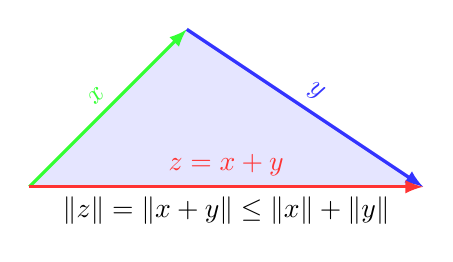
\begin{tikzpicture}[]
    % Punkte
    \coordinate (A) at (0,0) {};
    \coordinate (B) at (5,0) {};
    \coordinate (C) at (2,2) {};

    % Draw the triangle
    \path[fill=blue!10, fill=blue!10]  (A) -- (B) -- (C) -- (A);
    \draw[->, very thick,fill=gray!10, green!80, arrows={-latex}]  (A) -- (C) node[sloped,midway,above] {$x$};
    \draw[->, very thick,fill=gray!10, blue!80, arrows={-latex}]  (C) -- (B) node[sloped,midway,above] {$y$};
    \draw[->, very thick,fill=gray!10, red!80, arrows={-latex}]  (A) -- (B) node[sloped,midway,above] {$z = x + y$};
    \coordinate  (A) -- (B) node[sloped,midway,below] {$\|z\| = \|x+y\| \leq \|x\| + \|y\|$};



\end{tikzpicture}
\end{document}
